
\section{Kỹ thuật triển khai SVM}

\begin{frame}{Quy trình huấn luyện SVM điển hình}
  \begin{enumerate}
    \item \textbf{Thu thập và làm sạch dữ liệu}.
    \item \textbf{Tiền xử lý:}
      \begin{itemize}
        \item Chuẩn hóa đặc trưng (StandardScaler).
        \item Xử lý giá trị thiếu, mã hóa biến phân loại.
      \end{itemize}
    \item \textbf{Chọn kernel và mô hình:}
      \begin{itemize}
        \item Tuyến tính: \texttt{LinearSVC}.
        \item Phi tuyến: \texttt{SVC(kernel='rbf')}.
      \end{itemize}
    \item \textbf{Tối ưu siêu tham số} ($C$, $\gamma$) với Grid Search + Cross‑Validation.
    \item \textbf{Huấn luyện và đánh giá} trên tập test.
    \item \textbf{Triển khai} (lưu mô hình với \texttt{joblib} hoặc \texttt{pickle}).
  \end{enumerate}
\end{frame}

% ============================
% Tiền xử lý
% ===========================

\begin{frame}{Xử lý dữ liệu mất cân bằng}
  \begin{itemize}
    \item SVM cố gắng tối đa margin chung, có thể bỏ qua lớp thiểu số nếu không điều chỉnh.
    \item Giải pháp đơn giản trong sklearn: \texttt{class\_weight='balanced'}.
      \begin{itemize}
        \item Tự động tăng trọng số phạt $C$ cho các lớp ít mẫu.
      \end{itemize}
    \item Cũng có thể truyền dictionary trọng số tùy chỉnh: \texttt{class\_weight=\{0:1, 1:10\}}.
  \end{itemize}
  \begin{exampleblock}{Khi nào cần?}
    \begin{itemize}
      \item Tỉ lệ lớp chênh lệch lớn (ví dụ 1:10, 1:100).
      \item Bài toán cần recall cao cho lớp thiểu số (phát hiện gian lận, bệnh hiếm).
    \end{itemize}
  \end{exampleblock}
\end{frame}

\begin{frame}{Feature Scaling quan trọng như thế nào?}
  \begin{alertblock}{Tại sao SVM nhạy cảm với thang đo?}
    \begin{itemize}
      \item SVM dựa trên khoảng cách (margin) và tích vô hướng.
      \item Nếu một đặc trưng có giá trị lớn hơn hẳn, nó sẽ chi phối hàm mục tiêu và làm méo margin.
    \end{itemize}
  \end{alertblock}
  \begin{exampleblock}{Cách làm trong sklearn}
    \begin{itemize}
      \item Dùng \texttt{StandardScaler} để đưa mỗi đặc trưng về trung bình 0, độ lệch chuẩn 1.
      \item \textbf{Luôn} fit scaler trên tập huấn luyện, sau đó transform cho cả tập kiểm tra.
    \end{itemize}
  \end{exampleblock}
\end{frame}

\begin{frame}{Feature Scaling quan trọng như thế nào?}
  \begin{center}
    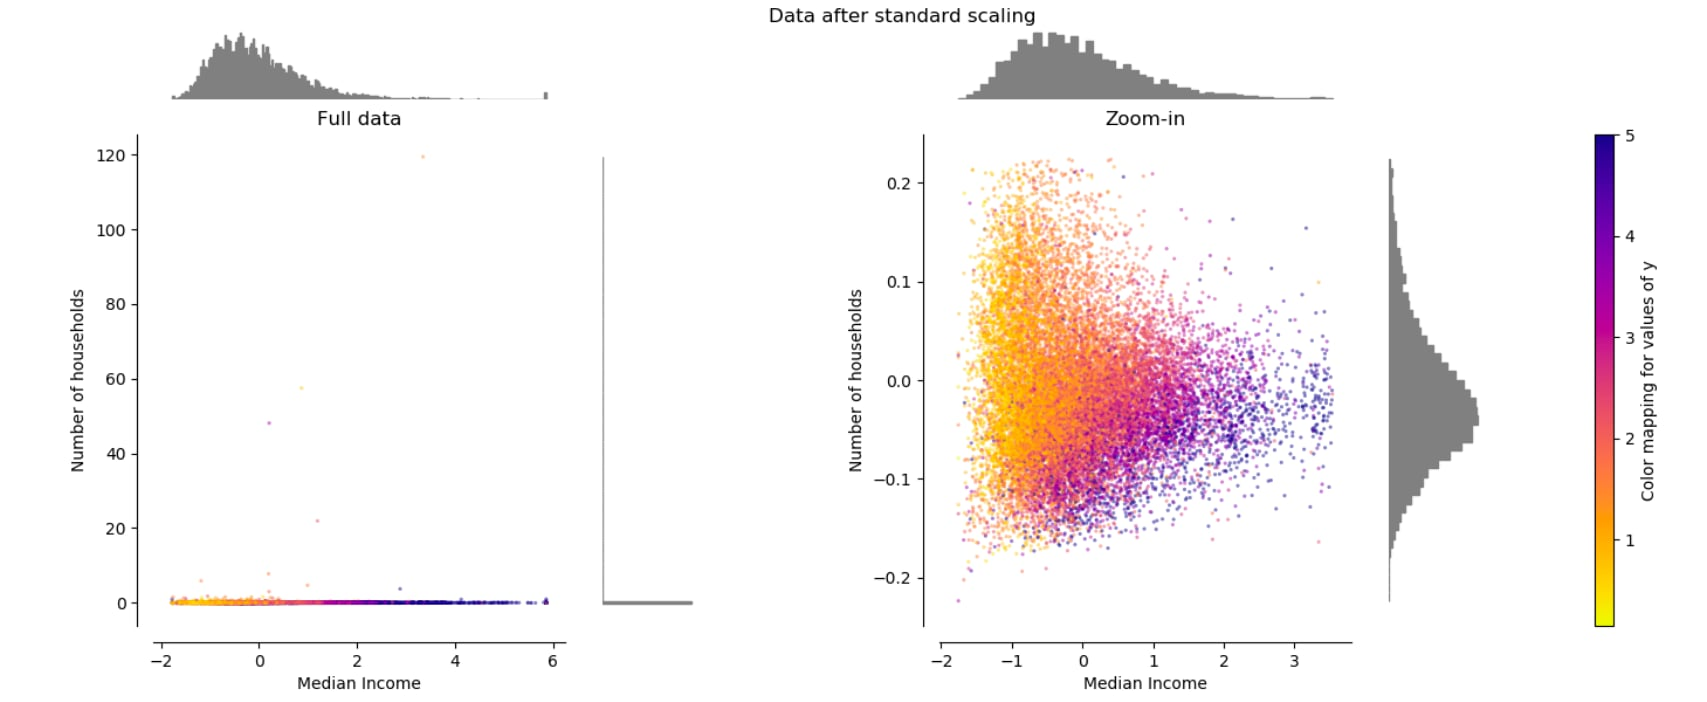
\includegraphics[width=\textwidth]{img/chapter_04/feature_scaling.jpg}
  \end{center}
\end{frame}

% ================================
% Triển khai SVM 
% ================================
\begin{frame}{LinearSVC vs SVC}
  \begin{columns}[T]
    \begin{column}{0.5\textwidth}
      \textbf{LinearSVC}
      \begin{itemize}
        \item Chuyên cho kernel tuyến tính.
        \item Tối ưu bằng thuật toán coordinate descent (nhanh, ít tốn RAM).
        \item Hỗ trợ dữ liệu thưa (sparse).
        \item \textbf{Dùng cho dữ liệu lớn} ($>10^5$ mẫu).
      \end{itemize}
    \end{column}
    \begin{column}{0.5\textwidth}
      \textbf{SVC(kernel='rbf')}
      \begin{itemize}
        \item Linh hoạt, xử lý ranh giới phi tuyến.
        \item Độ phức tạp $O(n^2)$ đến $O(n^3)$ về bộ nhớ/thời gian.
        \item Không phù hợp nếu $n > 10^4$–$10^5$.
        \item Có thể dùng \texttt{RBFSampler} để xấp xỉ kernel.
      \end{itemize}
    \end{column}
  \end{columns}
  \vspace{0.3cm}
  \begin{block}{Kinh nghiệm}
    \begin{itemize}
      \item Bắt đầu với LinearSVC (baseline). Nếu underfit, thử RBF.
      \item Với RBF, giảm số mẫu hoặc dùng xấp xỉ nếu dữ liệu quá lớn.
    \end{itemize}
  \end{block}
\end{frame}


\begin{frame}{Tối ưu $C$ và $\gamma$ với \texttt{GridSearchCV}}
  \begin{block}{Code mẫu}
    \begin{semiverbatim}
from sklearn.model\_selection import GridSearchCV

from sklearn.svm import SVC

param\_grid = \{

    'C': [0.1, 1, 10, 100],

    'gamma': [0.001, 0.01, 0.1, 1]

\}

grid = GridSearchCV(SVC(kernel='rbf'), param\_grid, cv=5)

grid.fit(X\_train\_scaled, y\_train)

print(grid.best\_params\_)
    \end{semiverbatim}
  \end{block}
  \begin{itemize}
    \item Luôn thực hiện cross‑validation (ví dụ cv=5) để đánh giá khách quan.
    \item Có thể dùng \texttt{RandomizedSearchCV} nếu không gian tham số quá lớn.
    \item Thời gian tìm kiếm tăng nhanh với số lượng mẫu – cân nhắc giảm lưới hoặc dùng tập con.
  \end{itemize}
\end{frame}


% ================================
% CÁC KHÍA CẠNH KHÁC
%================================
\begin{frame}{Lấy xác suất dự đoán từ SVM}
  \begin{itemize}
    \item Mặc định SVM chỉ trả về nhãn cứng ($\pm 1$) hoặc khoảng cách đến siêu phẳng.
    \item Để có xác suất (probability), cần bật \texttt{probability=True} khi khởi tạo SVC.
    \item Cơ chế: Platt scaling – hồi quy logistic trên output của SVM (tốn thêm thời gian huấn luyện).
  \end{itemize}
  \begin{block}{Lưu ý}
    \begin{itemize}
      \item Xác suất thu được có thể không được hiệu chuẩn tốt (calibrated) – cân nhắc dùng \texttt{CalibratedClassifierCV}.
      \item Không nên dùng probability nếu chỉ cần nhãn, vì làm chậm đáng kể.
    \end{itemize}
  \end{block}
\end{frame}

\begin{frame}{SVM với bài toán nhiều lớp (Multiclass)}
  \begin{itemize}
    \item SVM nguyên bản chỉ phân loại nhị phân.
    \item Để xử lý $K$ lớp ($K>2$), có hai chiến lược chính:
      \begin{enumerate}
        \item \textbf{One‑vs‑Rest (OvR)}: huấn luyện $K$ bộ SVM, mỗi bộ phân biệt một lớp với phần còn lại.
        \item \textbf{One‑vs‑One (OvO)}: huấn luyện $\binom{K}{2}$ bộ SVM, mỗi cặp lớp một bộ.
      \end{enumerate}
  \end{itemize}
  \begin{block}{Trong sklearn}
    \begin{itemize}
      \item \texttt{SVC} mặc định dùng \textbf{OvO} (phù hợp khi số lớp ít).
      \item \texttt{LinearSVC} mặc định dùng \textbf{OvR} (nhanh hơn cho nhiều lớp).
    \end{itemize}
  \end{block}
\end{frame}